\documentclass{standalone} %documento independente para figuras e tabelas
\usepackage{tikz} %usado para desenhar diagramas, gráficos
\usetikzlibrary{shapes, arrows} %adiciona funcionalidades extras ao TikZ para desenhar formas personalizadas (como retângulos, losangos) e setas personalizadas.

%---------------------------------------------
%Formas de todos os desenhos do Fluxograma
%---------------------------------------------

\tikzstyle{terminator} = [rectangle, draw, text centered, rounded corners, minimum height=2em] %O nó terá a forma de um retângulo; o contorno do nó será desenhado, ou seja, ele terá uma borda visível, O texto dentro do nó é centralizado horizontalmente, os cantos do retângulo serão arredondados, o que torna a forma mais suave, define a altura mínima do nó. A unidade "em" é uma medida relativa que depende do tamanho da fonte. Neste caso, a altura mínima será equivalente a 2X o tamanho da fonte.

\tikzstyle{process} = [rectangle, draw, text centered, minimum height=2em] %O nó terá a forma de um retângulo; o contorno (borda) do retângulo será desenhado, ou seja, terá uma borda visível, o texto dentro do nó será centralizado horizontalmente, define a altura mínima do nó. A unidade em é relativa ao tamanho da fonte, então o nó terá uma altura mínima de 2 vezes o tamanho da fonte.

\tikzstyle{decision} = [diamond, draw, text centered, minimum height=2cm] %O nó terá a forma de um losango, o contorno do losango será desenhado, o texto dentro do losango será centralizado, define a altura mínima do losango como 2 cm.

\tikzstyle{data}=[trapezium, draw, text centered, trapezium left angle=60, trapezium right angle=120, minimum height=2em] %Define o formato como um trapézio, o contorno do trapézio será desenhado, o texto dentro do trapézio será centralizado, o ângulo do lado esquerdo do trapézio será de 60º, o ângulo do lado direito será de 120 graus, garantindo um formato assimétrico, define a altura mínima do trapézio como 2 vezes o tamanho da fonte.

\tikzstyle{connector} = [draw, -latex'] %Desenha a linha do conector, define que a seta será uma seta no estilo Latex e será desenhada no final do conector (apontando na direção do fluxo do diagrama).
%---------------------------------------------
\begin{document}

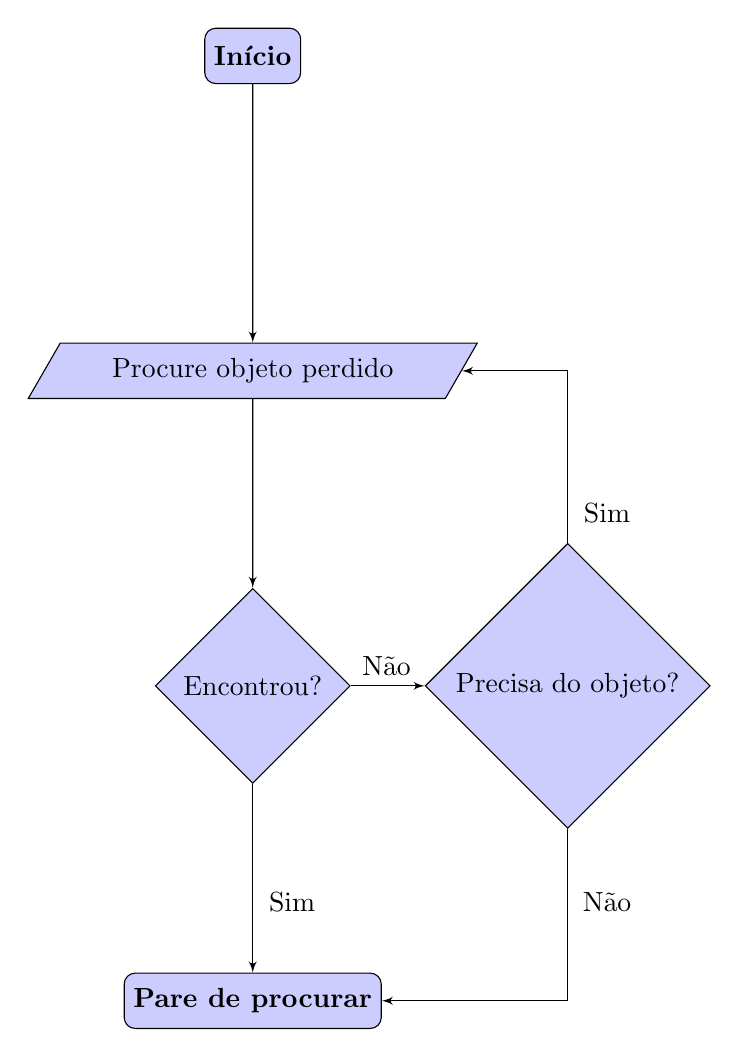
\begin{tikzpicture}[node distance=4cm] %ambiente de desenho com distanciamento de 4cm entre cada figura dentro do diagrama

%---------------------------------------------
%Todas as formas geométricas usadas no diagrama
%---------------------------------------------

\node [terminator, fill=blue!20] (inicio) {\textbf{Início}}; 
%retângulo inicial, topo da página, definido na cor azul com transparência de 20 %

\node [data, fill=blue!20, below of=inicio] (data) {Procure objeto perdido};
%trapézio abaixo do início, definido na cor azul com transparência de 20 %

\node [decision, fill=blue!20, below of=data] (decisao) {Encontrou?};
%losango abaixo do trapézio, definido na cor azul com transparência de 20 %

\node [decision, fill=blue!20, right of=decisao] (decisao2) {Precisa do objeto?};
%losango ao lado direito do primeiro losango, definido na cor azul com transparência de 20 %

\node [terminator, fill=blue!20, below of=decisao] (fim) {\textbf{Pare de procurar}};
%retângulo abaixo do primeiro losango, definido na cor azul com transparência de 20 %

%---------------------------------------------
%Legendas "Sim" e "Não" das fechas dos losangos e posicionamento (x,y)
%---------------------------------------------
\node[draw=none] at (1.70, -7.75) (nao) {Não};
\node[draw=none] at (4.5, -5.80) (sim) {Sim};

\node[draw=none] at (4.5, -10.75) (nao) {Não};
\node[draw=none] at (0.5, -10.75) (sim) {Sim};


%---------------------------------------------
%Conexão e flechas do Fluxograma
%---------------------------------------------
\path [connector] (inicio) -- (data);
\path [connector] (data) -- (decisao);
\path [connector] (decisao) -- (decisao2);
\path [connector] (decisao2) |- (data);
\path [connector] (decisao) -- (fim);
\path [connector] (decisao2) |- (fim);

\end{tikzpicture}


\end{document}
